\section{Kinetyka fizyczna}
\subsection{Równania transportowe Własowa [Vlasova] i Boltzmana}
Funkcja rozkładu $\f$ na przestrzeni $\mu,\ \dim[\mu]=6.$
\begin{equation} \f d^3rd^3p = \f d^6\omega \implies d^6\omega 
= d^3rd^3p \end{equation}
\begin{equation} \int d^3rd^p\f = N(t) \end{equation}
Dalej dla uproszczenia piszemy samo $N$ pamiętając o zależności czasowej.\\

\textbf{Dla gazu \underline{jednorodnego}:}
$$ \int d^3rd^3p \f = \int d^3rd^3pf(\vec{p},t) = V \int d^3p f(\vec{p},t)=N.$$
\begin{equation}
\int d^3p f(\vec{p},t) = \frac{N}{V} = n \mbox{ - koncentracja cząstek.}
\end{equation}
Oraz
\begin{equation}
N = \frac{\mbox{objętość układu}}{\mbox{objętość na jedną cząstkę}} \equiv 
\frac{V}{v}.
\end{equation}
Dla małego układu 
\begin{equation}
v=\frac{4}{3} \pi r_s^3 ,
\end{equation}
gdzie $r_s$ to promień kulki w jakiej możemy zamknąć jedną cząstkę. Stąd
$$ n = \frac{V}{v} \implies v=\frac{V}{N} = \frac{1}{n}$$
$$ \frac{4}{3} \pi r_s^3 = \frac{1}{n} \implies r_s = \left[ \frac{3}{4\pi n}
\right]^{1/3} \propto n^{-1/3}.$$
\begin{center}
\begin{minipage}{0.3\textwidth}
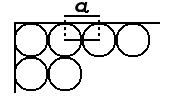
\includegraphics[width=5cm]{kuleczki_z_atomami.png}
\end{minipage}
\begin{minipage}{0.4\textwidth}
średnia odległość $a=2r_s$ \\
między cząsteczkami w gazie \\
o koncentracji $n$ \\
$$a \propto n^{-1/3}$$ \vspace{-5mm}\\
\end{minipage}
\end{center}

\textbf{Dla gazu \underline{niejednorodnego}:}
\begin{equation}
\int d^3rd^3\f = \int d^3r n(\vec{r}) = N \implies n(\vec{r}) 
\mbox{ - gęstość cząstek w } \vec{r}.
\end{equation}
%%%%%%%%%%%%%%%%%%%%%%% RYSUNEK %%%%%%%%%%%%%%%%%%%%%%%%%%%%%%%%%%%%%%%%%%%%%%%%%%%%
Funkcja rozkładu $f\rpt$. 

Zmiana położenia: efekty dryfowe

Zmiana pędu: efekty polowe

(pomijamy zderzenia)

$$ \Delta t:
\begin{cases} r \to & r+\Delta r \\
				p \to & p+\Delta p\end{cases}$$
$$ f(\vec{r}+\Delta\vec{r},\vec{p}+\Delta\vec{p},t+\Delta t) \simeq 
f\rpt +\nab{r} f\rpt \Delta r + \nab{p} f\rpt + \partial_t f\rpt $$
$$\dfrac{f(\vec{r}+\Delta\vec{r},\vec{p}+\Delta\vec{p},t+\Delta t)-f\rpt}{\Delta t}
\simeq \nab{r} f\rpt \frac{\Delta r}{\Delta t} + \ldots
$$
Przy $\Delta t \to 0$:
$$\dfrac{d}{dt} f\rpt = \nab{r} f\rpt \dfrac{d}{dt} \vec{r}(t) + \nab{p} f\rpt 
\dfrac{d}{dt} \vec{p}(t) + \partial_t f\rpt.$$
\begin{itemize}
\item ujęcie newtonowskie
$$\dfrac{d}{dt} f \rpt = \nab{r}f\rpt\cdot\underbrace{\vec{v}(t)}_{\mbox{prędkość
cz.}} +\nab{p}f\rpt\cdot\underbrace{\vec{F}(\vec{r})}_{\mbox{siła}}+\partial_t f\rpt$$
\item ujęcie hamiltonowskie
$$\dfrac{d}{dt} f\rpt = \nab{r} f\rpt \nab{p} H\rpt - \nab{p}f\rpt \nab{r}H\rpt +
\partial_t f\rpt = \{ f\rpt,H\rpt \} + \partial_t f\rpt.$$
Wzdłuż trajektorii fazowej $\frac{d}{dt}f\rpt =0$ [tw. Liouville'a].
\end{itemize}
\subsubsection{Równanie Własowa}
\begin{equation}
\vec{v}(t) \nab{r} \rpt + \vec{F}(\vec{r}) \nab{p}f\rpt +\partial_t f\rpt =0
\end{equation}
lub w innej postaci
\begin{equation}
\partial_t f\rpt = \{ H\rpt,f\rpt\}.
\end{equation}
\textbf{Opór Shavina - Maxwella}
%%%%%%%%%%%%%%%%%%%%%%% RYSUNEK %%%%%%%%%%%%%%%%%%%%%%%%%%%%%%%%%%%%%%%%%%%%%%%%%%%%
\begin{center}
Równanie Własowa $\equiv$ bezzderzeniowe równanie Boltzmana
\end{center}
\textbf{Zagadnienie Własowa-Pissona}
$$\begin{cases}
\vec{v}(t) \nab{r} \rpt + \vec{F}(\vec{r}) \nab{p}f\rpt +\partial_t f\rpt =0&\\
\nabla \vec{E} \arg = \left< \rho \arg \right>  \qquad \leftarrow \mbox{z uśrednieina teorii Lorenza}.& 
\end{cases}$$
Zakładane oddziaływania są zderzeniami. Zakładamy, że zderzenia są:
\begin{enumerate}
\item elastyczne i mają charakter podwójny (binarny)
\item kontaktowe, a w ich wyniku występuje jedynie zmiana pędu
%%%%%%%%%%%%%%%%%%%%%%% RYSUNEK %%%%%%%%%%%%%%%%%%%%%%%%%%%%%%%%%%%%%%%%%%%%%%%%%%%%
\end{enumerate}
\subsubsection{Klasyczny gaz rozrzedzony}
Klasycznym gazem rozrzedzonym nazywamy gaz cząstek klasycznych w którym zachodzą jedynie zderzenia binarne.
\begin{itemize}
\item[] $r_0$ - rozmiar liniowy cząstek
\item[] $l$ - średnia droga swobodna
\item[] $L$ - rozmiary liniowe układu
\end{itemize}
Charakterystyczna skalarna długość 
\begin{enumerate}
\item transport dyfuzyjny: $r_0 \ll l \ll L$
%%%%%%%%%%%%%%%%%%%%%%% RYSUNEK %%%%%%%%%%%%%%%%%%%%%%%%%%%%%%%%%%%%%%%%%%%%%%%%%%%%
\item transport balistyczny: $r_0 \ll L \ll l$
%%%%%%%%%%%%%%%%%%%%%%% RYSUNEK %%%%%%%%%%%%%%%%%%%%%%%%%%%%%%%%%%%%%%%%%%%%%%%%%%%%
\item lokalizacja: $r_0 \approx l < L$
%%%%%%%%%%%%%%%%%%%%%%% RYSUNEK %%%%%%%%%%%%%%%%%%%%%%%%%%%%%%%%%%%%%%%%%%%%%%%%%%%%
\end{enumerate}
Średnia droga swobodna to średnia odległość przebyta przez cząstkę pomiędzy kolejnymi zderzeniami.
\begin{equation}
l=\dfrac{1}{n\sigma},
\end{equation}
gdzie $\sigma$ - przekrój czynny.
%%%%%%%%%%%%%%%%%%%%%%% RYSUNEK %%%%%%%%%%%%%%%%%%%%%%%%%%%%%%%%%%%%%%%%%%%%%%%%%%%%
\subsection{Zespoły statysyczne i przestrzeń fazowa $\Gamma$}

